
\documentclass[12pt]{amsart}
\usepackage{geometry} % see geometry.pdf on how to lay out the page. There's lots.
\geometry{a4paper} % or letter or a5paper or ... etc
% \geometry{landscape} % rotated page geometry
\usepackage{multirow}
\usepackage{graphicx}

\usepackage{caption}

\usepackage[noend]{algpseudocode}

\usepackage{algorithmicx,algorithm}

% See the ``Article customise'' template for come common customisations

\title{Numerical Scheme And Hierarchically Solver For Anisotropic Poisson Equation With First Boundary Condition On Square Domain}
\author{Yiping Lu}
\date{} % delete this line to display the current date

%%% BEGIN DOCUMENT
\begin{document}
	
	

\maketitle
\begin{center}
	\small{luyiping9712@pku.edu.cn\\School of Mathematic Science, Peking University.\\No.5 Yiheyuan Road Haidian District,Beijing,P.R.China 100871.\\}
\end{center}

This lecture note is the report of the project of \textbf{Numerical Algebra(2017-2018Autumn)} instructed by Prof. Jun Hu at Peiking Univ.

\section{Numercial Schemes For Heat Equation With First Boundary Condition}

In this report we consider the following anisotropic problem:

\begin{align*}
\Delta_\epsilon u = u_{xx}+\epsilon u_{yy}=f,u|_{\partial D \times(0,1]}=0
\end{align*}

Here $D=(0,1)\times(0,1)$ is a square domain on the plane.

If we suggest the solution is $u(x,y)=\sin(\pi x)\sin(\pi y)$, so that$f(x,y)=-(1+\epsilon)\pi^2\sin(\pi x)\sin(\pi y)$


\subsection{Numerical Methods}


In this report we utilize the five point finite difference scheme, that is to say $\Delta_\epsilon$ is approximated by



\begin{align*}
\frac{U_{j+1,k}-2U_{j,k}+U_{j-1,k}}{h_x^2} + \epsilon \frac{U_{j,k+1}-2U_{j,k}+U_{j,k-1}}{h_y^2}
\end{align*}



 The local truncation error can be easily proved that has the formula $Tu(x,y)=-\frac{1}{12}(u_{xxxx}(x,y)h_x^2+\epsilon u_{yyyy}(x,y)h_y^2)+O(h_x^4+h_y^4)$

Consider the maximal principle which can be formatted as following:

\textbf{Theorem(Maximal Principle)} For the finite difference scheme $L_h$ defined as

\begin{align*}
L_hU_j = \sum_{i\in J\setminus  \{j\}}c_{i,j}U_i-c_jU_j
\end{align*} 

satisfies

\begin{itemize}
\item $J_D\not=\emptyset$ and $J=J_\Omega \cup J_D$ is connected
\item for every $j\in J_\Omega$ we have $c_j,c_{i,j}>0$ and $c_j\ge \sum_{i\in D_{L_h}(j)}c_{i,j}$
\end{itemize}

Then

\begin{align*}
\max_{i\in J_\Omega} U_i \le \max\{\max_{i\in J_D}U_i,0\}
\end{align*}

It's easy to find that the numerical scheme satisfies the maximal principle, that is to say our scheme is stable under norm $||\cdot||_\infty$.






\section{Hierarchically Numerical Linear Algebra Method For The Problem}

This section is based on Volker John's Lecture nots on multigrid and Jinchao Xu's review paper 'Iterative methods: by space decomposition and subspace correction'.

\subsection{Detialed Investigation of Classical Iterative Schemes}
\subsubsection{General Aspects of Classical Iterative Scheme}
To solve the linear system $Au=f$ we can give a general approach: let $A=M-N$ , the iterative scheme can be formula as
\begin{align*}
u^{*}&=M^{-1}Nu+M^{-1}f:=Su+M^{-1}f\\
u^{(m+1)}&=\omega u^*+(1-\omega)u^{(m)}
\end{align*}

such that $u^{(m+1)}=(\omega S+(1-\omega)I)u^{(m)}+\omega M^{-1}f$ and we have residual equation $Se^{(m)}=e^{(m+1)}$

This scheme can conclude Damped Jacobi method and the SOR method.
\subsubsection{Converge Analysis}
First apply Discrete Fourier Method to analysis the scheme. For a give function $b$ on $[0,1]$, we can expanded in the form
\begin{align*}
b(x)=\sum_{k=1}^{\infty} b_k\sin(k\pi x)
\end{align*}

Here we can analyze $u^{(0)}=(u_1^{(0)},\cdots,u_{N-1}^{(0)})^T,u_j^{(0)}=\sin(\frac{jk\pi}{N})(j,k=1,\cdots,N-1)$  This discrete Fourier modes are also the \textbf{eigenvectors} of the matrix $A$. 
\begin{itemize}
	\item For $1\le k <N/2$ are called the low frequency or smooth modes.
	\item For $N/2\le k\le N-1$ are called high frequency or oscillating modes.
\end{itemize}

There are several important observation
\begin{itemize}
	\item On a fixed grid, there is a good damping of the high frequency errors whereas there is almost no damping of the low frequency errors.
	\item For a fixed wave number, the error is reduced on a coarser grid better than on a finer grid.
	\item The logarithm of the error decays linearly.
\end{itemize}

\textbf{damped Jacobi methods}

For damped Jacobi methods the iteration matrix is $S_{jac,\omega}=I-\omega D^{-1}A=I-\frac{\omega h}{2}A$, it has eigenvalue

\begin{align*}
\lambda_k(S_{jac,\omega})=1-\frac{\omega h}{2}\lambda_k(A)=1-2\omega\sin^2(\frac{k\pi h}{2})
\end{align*}

It is easy to see that \textbf{damped Jacobi method converges fastest for $\omega=1$} which only need to solve a  min-max problem and the error has the form $e^{(n)}=\sum_{k=1}^{N-1} c_k\lambda_k(S_{jac,\omega})w_k$


\textbf{SOR methods}

The first thing we need to calculate is the eigenvalue of $S_{GS}$:

\begin{align*}
\lambda_k(S_{GS})=\cos^2(\frac{k\pi}{N})
\end{align*}

\begin{proof}
	Inserting the decomposition of $S_{GS}$ gives
	\begin{align*}
	-(D+L)^{-1}Uw_k = \lambda_k(S_{GS})w_k \Leftrightarrow \lambda_k(S_{GS})(D+L)w_k=-Uw_k
	\end{align*}
	
	Considering the model problem and inserting the representation of the $k$-th eigenvector 
	\begin{align*}
	\lambda_k(S_{GS})\left[2 \lambda_k(S_{GS})^{1/2}\sin(\frac{jk\pi}{N}) -\sin(\frac{(j-1)k\pi}{N}) \right]=(\lambda_k(S_{GS}))^{(j+1)/2}\sin(\frac{(j+1)k\pi}{N})
	\end{align*}
	if we let
	\begin{align*}
	\lambda_k(S_{GS})=\cos^2(\frac{k\pi}{N})
	\end{align*}
	It becomes a well-known relation
	\begin{align*}
	2\sin(\frac{\alpha+\beta}{2})\cos(\frac{\alpha-\beta}{2})=\sin \alpha+\sin\beta
	\end{align*}
	with $\alpha=(j+1)k\pi/N,\beta=(j-1)k\pi/N$
\end{proof}
With the calculated eigenvalue the converge analysis is so naive that anyone could do it.
\subsection{Multigrid Methods}

Above all, I want to say the multigrid methods may not be the fastest method in solving the implicit scheme of $u_t=\Delta u$ but is suitable for Laplace equation $\Delta u=f$
\subsubsection{Grid Transfer}

We give some properties of the restriction and interpolation operator. $I_{2h}^h,I_h^{2h}$
\begin{itemize}
	\item $I_{2h}^{h}$ is full rank and the trivial kernel
	\item $I_h^{2h}=2(I_h^{2h})^T$
	\item Dual Operator:$\left<I_{2h}^hv^{2h},r^h\right>_{V^h,(V^h)^*}=\left<v^2h,I_h^{2h}r^h\right>_{V^{2h},(V^{2h})^*}$
	\item For the 1D model problem we have $A^{2h}=I_h^{2h}A^hI_{2h}^h$(Galerkin Projection)
\end{itemize}

\subsubsection{Two Level Methods}
The algorithm is give as
\begin{itemize}
	\item $A^{2h}u^{2h}=f^{2h}$ compute an approximation $v^{2h}$ and compute the residual $r^{2h}=f^{2h}-A^{2h}v^{2h}$
	\item Solve the coarse grid equation $A^he^h=I_{2h}^h(r^{2h})$
	\item $v^h=v^h+I_h^{2h}(e^{h})$
\end{itemize}



\textbf{Iteration Matrix.} Let $S_{sm}$ be the iteration matrix of the smoother.  The calculation can be seen at \textbf{Multilevel Method} in the next section. The iteration matrix can be given as
\begin{align*}
S_{2lev} = (I-I_{h}^{2h}(A^h)^{-1}I_{2h}^hA^h)S_{sm}
\end{align*}

\textbf{Converge Analysis.}
Here we give some definition used in the converge analysis
\begin{itemize}
	\item \textbf{Smoothing property}
	\begin{align*}
	|||A^hS_{sm}|||\le Ch^{-\alpha}
	\end{align*}
	\item \textbf{Approxiamation property}
	\begin{align*}
	|||(A^{2h})^{-1}-I_h^{2h}(A^h)^{-2}I_{2h}^h|||\le C_ah^\alpha
	\end{align*}
\end{itemize}

Following the above two property we can give a converge speed to the algorithm as $|||S_{2lev}|||\le CC_a$.For every specific algorithm used in the multi-grid framework, you should analyze the above two properties.


\subsubsection{Multigrid}

The W-multigrid can be analyzed by the processing before maybe it can be the appendix of my report for Numerical Algebra. The V-multigrid can be analyzed as a multi-level subspace correction algorithm. 

\subsection{Subspace Correction}

Solving the linear equation can be seen as the following three steps:
\begin{itemize}
	\item $r^{old}=f-Au^{old}$
	\item $\hat e =Br^{old}$ with $B \approx A^{-1}$
	\item $u^{new}=u^{old}+\hat e$
\end{itemize}
The choice of $B$ is the core of this type of alogrithm. The point is to choice $B$ by solving appropriate subspace problems. The subspaces are provided by a decomposition of $V$: $V=\sum_{i=1}^JV_i$. Here $V_i$ are the subspaces of $V$. Assume $A_i:V_i\rightarrow V_i$ is restriction operator of $A$ on $V_i$, then we can let $B=R_i\approx A_i^{-1}$ \textbf{Multigrid and domain decomposition methods can be viewed under this perspective.} In this section we only consider the linear iteration methods like $u^{k+1}=u^{k}+B(f-Au^k)$.

Here $B$ is a approximate of the inverse matrix $A^{-1}$ and the sufficient condition for the convergence of the scheme is
\begin{align*}
\left|\left|I-BA\right|\right|_A<1
\end{align*}

which can be seen in the appendix of the ppt for Iteration Methods.

\subsubsection{Subspace correction and subspace equations}
For subspace decomposition$V=\sum_{i=1}^JV_i$, for each $i$ we define $Q_i,P_i:V\rightarrow V_i$ and $A_i:V_i\rightarrow V_i$ by 
\begin{align*}
(Q_iu,v_i)=(u,v_i),(P_iu,v_i)_A=(u,v_i)_A,(A_iu_i,v_i)=(Au_i,v_i)
\end{align*}

Here $P_i,Q_i$ are both orthogonal projections and $A_i$ is the restriction of $A$ on $V_i$ and is SPD. It follows the definition that $A_iu_i=f_i$ with $u_i=P_iu,f_i=Q_i f$ At the same time we use $R_i$ to represent an approximate inverse of $A_i$ in certain sense. Thus an approximate solution is given by $\hat u_i = R_if_i$

\textbf{Basic Idea:}Consider the residual equation $Ae=r^{old}$ Instead of $u=u^{old}+e$ we solve the restricted equation to each subspace $A_ie_i=Q_ir^{old}$, while using the subspace solver $R_i$ described earlier equally the process can be written as $\hat e_i=R_iQ_ir^{old}$


\textbf{PSC:Parallel Subspace Correction.} Similar to Jacobi Methods.(When $V=\sum span(\{e_i\})$, PSC becomes Jacobi)

An update of the approximation of $u$ is obtained by
\begin{align*}
u^{new}=u^{old}+\sum_{i=1}^J \hat e_i
\end{align*}
which can be equally written as 
\begin{align*}
u^{new}=u^{old}+B(f-Au^{old})
\end{align*}
where $B=\sum_{i=1}^J  R_iQ_i$

\textbf{Lemma.} The operator $B$ is SPD.
\begin{proof}
	\begin{align*}
	(Bv,v)=\sum_{i=1}^J(R_iQ_iv,Q_iv)\ge 0
	\end{align*}
	
	And the symmetry of $B$ follows from the symmetry of $R_i$
\end{proof}

As a simple corollary, $B$ can be used as a preconditioner liker CG methods.  .(When $V=\sum span(\{e_i\})$, $B$ becomes the simplest preconditioner $diag(a_{11}^{-1},\cdots,a_{nn}^{-1})$

\textbf{SSC:Successive Subspace Correction.} Similar to Gauss-Seidel Methods.(When $V=\sum span(\{e_i\})$, SSC becomes G-S)
This method is used as

\begin{align*}
v^1&=v^0+R_1Q_1(f-Av^0)\\
v^2&=v^1+R_2Q_2(f-Av^1)\\
\cdots
\end{align*}

Formerly the algorithm can be written as $u^{(k+i)/J}=u^{(k+i-1)/J}+R_iQ_i(f-Au^{(k+i-1)/J})$

Let $T_i=R_iQ_iA$ Then we have
\begin{align*}
u-u^{(k+i)/J}=(I-T_i)(u-u^{(k+i-1)/J})
\end{align*}

A successive application of this identity yields
\begin{align*}
u-u^{k+1}=E_J(u-u^k)
\end{align*}

where $E_J=(I-T_J)(I-T_{J-1})\cdots(I-T_1)$

Like SOR method we can also have an algorithm as$u^{(k+i)/J}=u^{(k+i-1)/J}+\omega R_iQ_i(f-Au^{(k+i-1)/J})$


\textbf{Multilevel Methods.} Multilevel algorithms are based on a nested sequence of subspaces
\begin{align*}
M_1\subset M_2\subset\cdots\subset M_J=V
\end{align*}

\textbf{Algorithm.}
\begin{itemize}
	\item Correction:$v^1=\hat B_{k-1}\hat Q_{k-1}g$
	\item Smoothing:$\hat B_kg=v^1+\hat R_k(g-\hat A_kv^1)$
\end{itemize}

Next we want to show that \textbf{the multilevel method is equivalent to the SSC algorithm.}

Suppose $M_k=\sum_{i=1}^k V_i$ It is easy to show that the two algorithm is equivalent.



\subsubsection{Converge Theory}
\begin{itemize}
	\item For PSC we need to estimate the condition number of $T=BA=\sum_{i=1}^JT_i$.
	\item For SSC we need to estimate $\left|\left|E_J\right|\right|_A<1$
\end{itemize}

We define two parameters $K_0,K_1$ at the beginning of the section.
\begin{itemize}
	\item For any $v=\sum_{i=1}^Jv_i\in V$ we have $\sum_{i=1}^J(R_i^{-1}v_i,v_i)\le K_0(Av,v)$
	\item For any $u_i,v_i$ we have
	\begin{align*}
	\sum_{\left\{1,2,\cdots,J\right\}^2} (T_iu_i,T_jv_j)\le K_1(\sum_{i=1}^J(T_iv_i,v_i)_A)^{1/2}(\sum_{j=1}^J(T_jv_j,v_j)_A)^{1/2}
	\end{align*}
\end{itemize}
\textbf{PSC.\\}

\textbf{Theorem.} Assume that $B$ is the SSC preconditioner then
\begin{align*}
\kappa(BA)\le K_0K_1
\end{align*}
\begin{proof}
	Follow directly from the definition of $K_1$ that
	\begin{align*}
	\left|\left|Tv\right|\right|_A^2=\sum_{i,j=1}^J(T_iv,T_jv)_A\le K_1(Tv,v)_A\le K_1\left|\left| Tv\right|\right|_A\left|\left|v\right|\right|_A
	\end{align*}
	which implies $\lambda_{\max}(BA)\le K_1$
	
	At the same time
	\begin{align*}
	(v,v)_A=\sum_{i=1}^J(v_i,P_iv)_A&\le\sum_{i=1}^J\left(R_i^{-1}v_i,v_i\right)^{1/2}\left(R_iA_iP_iv_i,v\right)_A^{1/2}\\
	&\le \left(\sum_{i=1}^J\left(R_i^{-1}v_i,v_i\right)\right)^{1/2}\left(\sum_{i=1}^J\left(R_iA_iP_iv_i,v\right)_A\right)^{1/2}\\
	&\le \sqrt{K_0} \left|\left|v\right|\right|_A(Tv,v)_A^{1/2}
	\end{align*}
	
	which implies $\lambda_{\min}(BA)\ge K_0$ and $\kappa(BA)\le K_0K_1$
	
\end{proof}

\textbf{SSC.\\}

For $E_i=(I-T_i)(I-T_{i-1})\cdots(I-T_1)$ and $E_0=I$ Then
\begin{align*}
I-E_i=\sum_{j=1}^i T_jE_{j-1}
\end{align*}

\textbf{Lemma.}
\begin{align*}
(2-\omega_1)\sum_{i=1}^J(T_iE_{i-1}v,E_{i-1}v)_A\le \left|\left|v\right|\right|_A^2-\left|\left|E_Jv\right|\right|_A^2
\end{align*}

\begin{proof}
	\begin{align*}
	\left|\left|E_{i-1}v\right|\right|_A^2-\left|\left|E_{i}v\right|\right|_A^2 &= \left|\left|T_{i}E_{i}v\right|\right|_A^2+2(T_iE_{i-1}v,E_iv)_A\\
	&=(T_iE_{i-1}A,T_iE_{i-1}v)_A+2(T_i(I-T_i)E_{i-1}v,E_{i-1}v)_A\\
	&=((2I-T_i)T_iE_{i-1}v,E_{i-1}v)_A\ge (2-\omega_1)(T_iE_{i-1}v,E_{i-1}v)_A
	\end{align*}
\end{proof}


\textbf{Theorem.}
\begin{align*}
\left|\left|E_J\right|\right|_A^2\le 1-\frac{2-\omega_1}{K_0(1+K_1)^2}
\end{align*}

\begin{proof}
	First it is easy to show that
	\begin{align*}
	\sum_{i=1}^J(T_iv,v)_A\le(1+K_1)^2\sum_{i=1}^J(T_iE_{i-1}v,E_{i-1}v)_A
	\end{align*}
	
	At the same time we have
	\begin{align*}
	\sum_{i=1}^J(T_iv,E_{i-1}v)_A\le \left(\sum_{i=1}^J(T_iv,v)_A\right)^{1/2}\left(\sum_{i=1}^J(T_iE_{i-1}v,E_{i-1}v)_A\right)^{1/2}
	\end{align*}
	and
	\begin{align*}
	\sum_{i=1}^J\sum_{j=1}^{i=1}(T_iv,T_jE_{j-1}v)_A\le K_1\left(\sum_{i=1}^J(T_iv,v)_A\right)^{1/2}\left(\sum_{i=1}^J(T_iE_{i-1}v,E_{i-1}v)_A\right)^{1/2}
	\end{align*}
	Combining these three formulas leads to the theorem.
\end{proof}

At last I want to introduce a prefect websit:http://www.mgnet.org/










\section{Numerical Results}

In this section, we will test several algorithms
\begin{itemize}
	\item G-S symmetric version
	\item Block G-S symmetric version
	\item Conjugate Gradient Method
	\item Conjugate Gradient Method Utlizing A V-cycle Multi grid method as a pre-conditioner
	\item Gauss Method
\end{itemize}

In order to do fair comparison, we will make the following comparison

\begin{itemize}
	\item Conjugate Gradient Vs Pre-Condition Conjugate Gradient
	\item G-S Vs Block G-S
\end{itemize}

For the solution is a solution of a PDE, I will using a new method to calculate the numerical error instead of the vector $l2-$norm.

First we will give a method to do the interpolation on a square $[0,1]\times[0,1]$. Using four polynomial $xy,x(y-1),y(x-1),(x-1)(y-1)$ as bases and that is to say

\begin{align*}
	f(x,y)=f(0,0)(x-1)(y-1)+f(1,0)x(1-y)+f(0,1)y(1-x)+f(1,1)xy
\end{align*}

Using this interpolation, we get a function interpolated by our value on the grid points. Then calculating the error in $l^2([0,1]\times[0,1])$ using a Gaussian integral method. That is to say our error is defined as

\begin{align*}
	\int_{[0,1]\times[0,1]} |\hat f-f_{true}|^2dx
\end{align*}

From Table\ref{numericalerror} we can see the numerical scheme is one order.

\begin{table}[h]
	\centering
	\caption{Error For The Numerical Scheme}
	\label{numericalerror}
	\begin{tabular}{llll}
		Grid Szie         & 128        & 256        & 512         \\
		\hline\hline
		Function l2 Error & 7.4e-10    & 5.8e-11    & \textbf{6.1e-12}     \\
		Vector l2 Error   & 0.00321316 & 0.00160693 & 0.000823503
	\end{tabular}
\end{table}

\begin{center}
	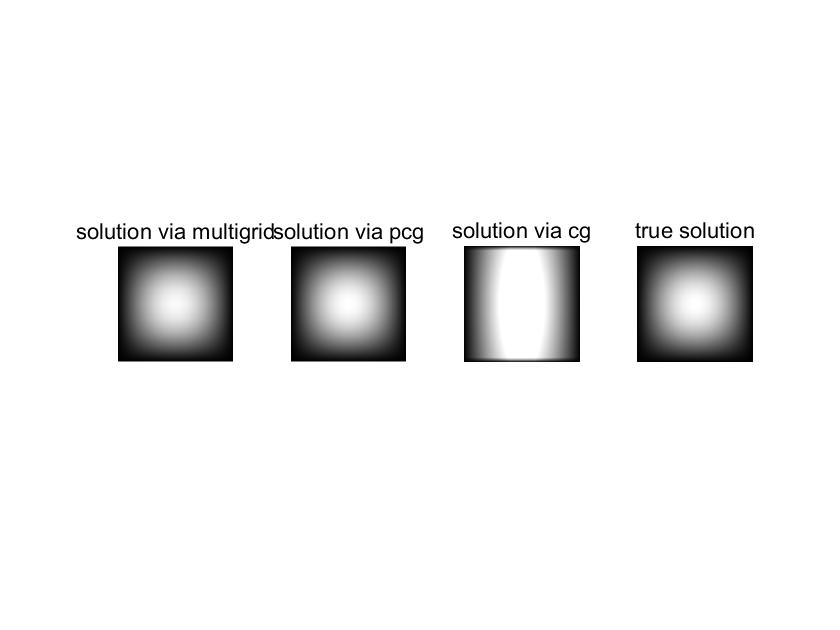
\includegraphics[width=5in]{solu.jpg}\\
	\textbf{Fig.} Solution of the anisotropic Poisson equation, when the diffusion coefficient is $\epsilon=1e-2$ (grid size=512, cg method has a max iteration number of 300.)
\end{center}



\subsection{CG VS PCG}

PCG is method of using preconditioning in conjugate gradient methods.


\begin{algorithm}[h]
	\caption{(Pre-conditioned Conjugate Gradient)} 
	\hspace*{0.02in} {\bf Input:} 
	pre-conditioner:$M$, initial guess $x_0$\\
	\begin{algorithmic}[1]
		\State $r_0=b-Ax_0$ 

		

		\While{Not converged}
		\State (Pre-condition)Solve equation $Mz_k=r_k$ (If no pre-condition method $z_k=r_k$)
		\State $k=k+1$
		\If{$k=1$} % If 语句,需要和EndIf对应
		\State $p_1=z_0$
		\Else
		\State $\beta_k=\frac{r_{k-1}^Tz_{k-1}}{r_{k-2}^Tz_{k-1}}$, $p_k=z_{k-1}+\beta_kp_{k-1}$
		\EndIf
		\State $\alpha_k=\frac{r_{k-1}^Tz_{k-1}}{p_k^TAp_k}$
		\State $x_k=x_{k-1}+\alpha_kp_k$, $r_k=r_{k-1}-\alpha_kAp_k$
		\EndWhile
		\State \Return $x_k$
	\end{algorithmic}
\end{algorithm}

In this section we utilize a V-cycle multi-grid method as the solve to pre-condition the problem. The converge speed is ploted as following.

\begin{table}[]
	\centering
	\caption{PCG Iteration Times and CPU Time. Termination condition is $||r_k||/||r_0||<1e-8$.}
	\label{pcg}
	\begin{tabular}{|l||lll|}
		\hline\hline
		Iteration Time & 128 & 256 & 512 \\ \hline\hline
		$\epsilon=1e0$            & 4/0.15   & 4/0.66   & 4   \\ \hline
		$\epsilon=1e-1$           & 6/0.22   & 6/0.96   & 6   \\ \hline
		$\epsilon=1e-2$          & 16/0.58  & 16/1.95  & 16  \\ \hline
		$\epsilon=1e-3$           & 39/1.07  & 42/4.88  & 43  \\ \hline
		$\epsilon=1e-4$           & 55/1.95  & 93/14.44  & 110 \\ \hline
	\end{tabular}
\end{table}

\begin{center}
	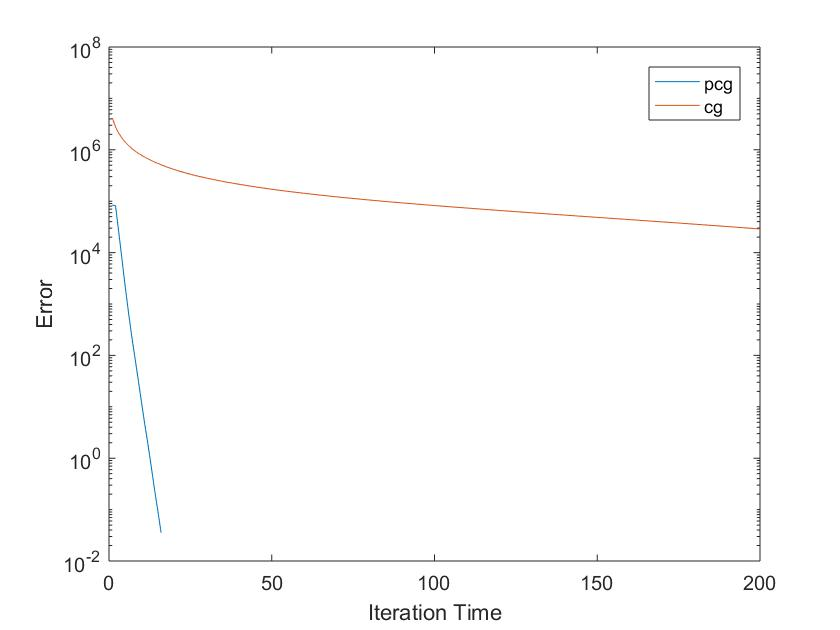
\includegraphics[width=2.5in]{plot.jpg}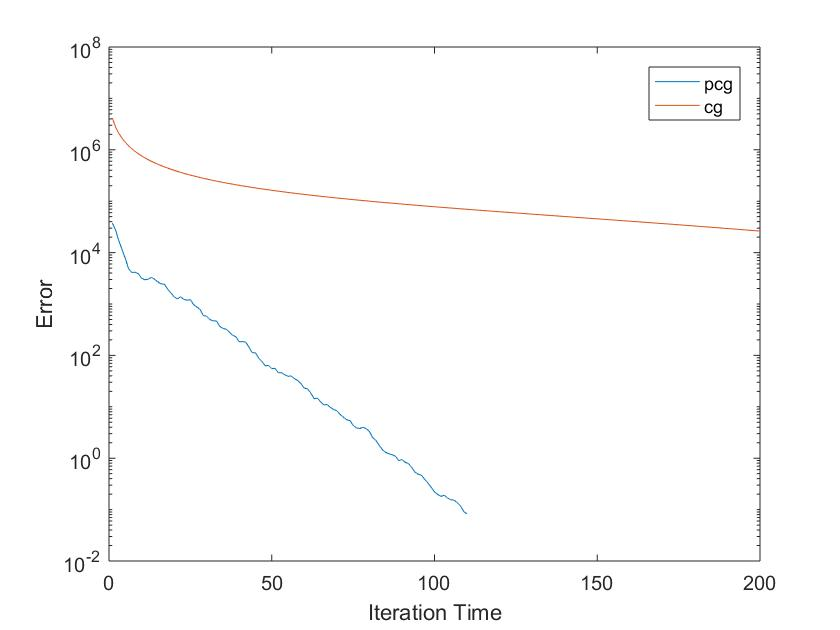
\includegraphics[width=2.5in]{plot2.jpg}\\
	\textbf{Fig.} The error(vector l2-norm)-iteration time plot.(grid size:512, $\epsilon=1e-2,1e-4$)
\end{center}

\subsection{Block G-s}

First, for the matrix can be written as

\begin{gather*}
\begin{bmatrix} 
A_{11}&A_{12}&\cdots&A_{1r}\\ 
A_{21}&A_{22}&\cdots&A_{2r}\\
\cdot &\cdot&&\cdot\\ 
\cdot &\cdot&&\cdot\\ 
\cdot &\cdot&&\cdot\\ 
A_{r1}&A_{r2}&\cdots&A_{rr}
\end{bmatrix}
\end{gather*}

here $A_{ij}$ is a $n_i\times n_j$ sub-matrix and $\sum n_i=n$. Rewrite $x=(x_1^T,x_2^T,\cdots,x_r^T)^T,b=(b_1^T,b_2^T,\cdots,b_r^T)^T$. Let $A=D_B-L_B-U_B$, here $D_B=diag(A_{11},A_{22},\cdots,A_{rr})$

Then the block G-S method can be consider as iteration for solving the equation in order
\begin{align*}
	A_{ii}x^{(k+1)}=b_i-\sum_{j=1}^{i-1}A_{ij}x^{(k+1)}_j-\sum_{j=i+1}^{r}A_{ij}x_j^{(k)}
\end{align*}


\begin{figure}[H]
	\begin{minipage}{0.48\linewidth}
		\centerline{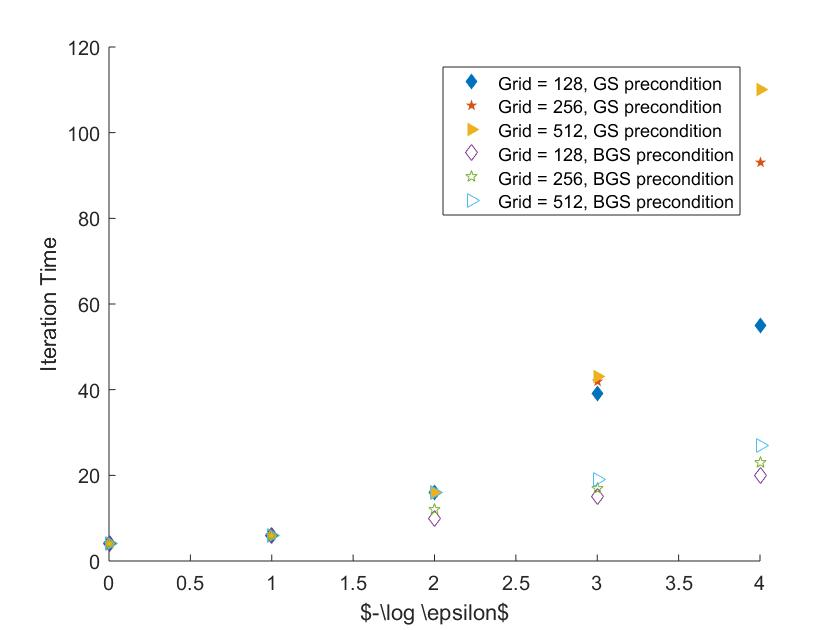
\includegraphics[width=9.0cm]{final.jpg}}
	\end{minipage}
	\hfill
	\begin{minipage}{.48\linewidth}
			\centering
			\begin{tabular}{|l|c|c|c|c|}\hline
				Setting&\multicolumn{2}{c|}{Iteration Time}&\multicolumn{2}{c|}{CPU Time}\\\hline\hline
				&G-S&Block G-S&G-S&Block G-S\\
				\hline\hline
				$\epsilon=1$&16428&8218&1.337&3.374\\
				\hline
				$\epsilon=1e-1$&15964&1462&1.296&0.596\\
				\hline
				$\epsilon=1e-2$&16108&180&1.306&0.079\\
				\hline
				$\epsilon=1e-3$&16334&34&1.296&0.017\\
				\hline
				$\epsilon=1e-4$&16646&14&1.328&0.008\\
				\hline
				$\epsilon=1e-5$&16692&\textbf{8}&1.318&\textbf{0.005}\\\hline\hline
			\end{tabular}
			
	\end{minipage}
	\caption{Iteration Times For G-S and Block G-S When Grid size is 64 and termination condition is $||r_k||/||r_0||<1e-6$ and comparison of being pre-conditioner.}
	\label{zrotate}
\end{figure}



\subsection{Partial Gauss Method}

In this section, we utilize the Gaussian elimination method to solve the linear equation. For the matrix have a bandwidth of $grid\_size$, we don't need to calculate the zero part. Moreover, the matrix is \textbf{dominant diagonally dominant}, \emph{the partial pivoting method is no longer needed here}. In short the algorithm can be listed as

\begin{algorithm}[h]
	\caption{(Partial Gaussian Elimination For Poisson Equation)} 
	
	\begin{algorithmic}[1]
		
		
		
		\For{k = 1:n-1}
		\State A(k+1:min(k+grid\_size,n),k)=A(k+1:min(k+grid\_size,n),k)/A(k,k);
		\State A(k+1:min(k+grid\_size,n),k+1:n)=A(k+1:min(k+grid\_size,n),k+1:n)-A(k+1:min(k+grid\_size,n),k)*A(k,k+1:n);
	
		\EndFor
		\State L=speye(n,n)+tril(A,-1);
		\State U=triu(A);
	
		\State \Return [L, U]
	\end{algorithmic}
\end{algorithm}


\begin{table}[h]
	\centering
	\caption{CPU Time \& Error By Partial Gauss Method}
	\label{gauss}
	\begin{tabular}{|l|lll|}
		\hline
		CPU Time/Error & 1e0            & 1e-2           & 1e-5           \\ \hline\hline
		16             & 0.13/3.617e-6  & 0.09/3.617e-6  & 0.08/3.617e-6  \\ \hline
		32             & 0.21/2.35e-7   & 0.17/2.35e-7   & 0.18/2.35e-7   \\ \hline
		64             & 10.52/1.687e-8 & 10.93/1.687e-8 & 10.58/1.687e-8 \\ \hline\hline
	\end{tabular}
\end{table}






\subsection{Heat Equation Solution}

We also made a test for the heat equation. We use several numerical methods to solve the PDE. We test the \textbf{explicit scheme, implicit scheme} and the \textbf{Crank-Nicolson Scheme}. For test, we utlize the initial condition $u(x,y,0)=\sin(\pi x)\sin(\pi y)$, this PDE can be easily solved with solution $u(x,y,t)=e^{-2\pi^2t}\sin(\pi x)\sin(\pi y)$

\subsubsection{Explicit Scheme} The forward explicit scheme can be simply written as

\begin{align*}
\frac{U_{j,k}^{m+1}-U_{j,k}^{m}}{h_t}=\frac{U_{j+1,k}^m-2U_{j,k}^m+U_{j-1,k}^m}{h_x^2} + \frac{U_{j,k+1}^m-2U_{j,k}^m+U_{j,k-1}^m}{h_y^2}
\end{align*}

\subsubsection{Implicit scheme} Here we consider the implicit scheme has the following formula which contains the Crank-Nicolson Scheme as a special case

\begin{align*}
\frac{U_{j,k}^{m+1}-U_{j,k}^{m}}{h_t}&=
(1-\theta)(\frac{\delta_x^2}{h_x^2}+\frac{\delta_y^2}{h_y^2})U_{j,k}^m+\theta(\frac{\delta_x^2}{h_x^2}+\frac{\delta_y^2}{h_y^2})U_{j,k}^{m+1}\\
&=
(1-\theta)(\frac{U_{j+1,k}^m-2U_{j,k}^m+U_{j-1,k}^m}{h_x^2} + \frac{U_{j,k+1}^m-2U_{j,k}^m+U_{j,k-1}^m}{h_y^2})+\\
&\theta (\frac{U_{j+1,k}^{m+1}-2U_{j,k}^{m+1}+U_{j-1,k}^{m+1}}{h_x^2} + \frac{U_{j,k+1}^{m+1}-2U_{j,k}^{m+1}+U_{j,k-1}^{m+1}}{h_y^2})
\end{align*}
For the Fourier wave $U_{j,k}^m=\lambda_\alpha^me^{i(\alpha_xx_j+\alpha_yy_k)}$,  we have

\begin{align*}
\lambda_\alpha=\frac{1-4(1-\theta)(\mu_x\sin^2\frac{\alpha_xh_x}{2}+\mu_y\sin^2\frac{\alpha_yh_y}{2})}{1+4\theta(\mu_x\sin^2\frac{\alpha_xh_x}{2}+\mu_y\sin^2\frac{\alpha_yh_y}{2})}
\end{align*}

In order to obtain the stability we need

\begin{align*}
2(\mu_x+\mu_y)(1-2\theta)\le 1, 0\le \theta\le \frac{1}{2}
\end{align*}

\textbf{Why Crank-Nicolson Scheme Choose $\theta=\frac{1}{2}$}

The local truncation error can be proof to be $O(h_t^2+h_x^2+h_y^2)$ when  $\theta=\frac{1}{2}$ and to be $O(h_t+h_x^2+h_y^2)$ when $\theta$ is other value.



\subsection{Performance of different schemes}  
In this section, all of the results is using \textbf{pcg} in order to get fast and robust solutions:


\begin{table}[!hbp]
	\begin{tabular}{|c|c|c|c|c|c|}
		\hline
		\hline
		Test & Space step & Time step & CN Scheme & Implicit Scheme&Explicit Scheme \\
		\hline
		1 & 1/512 & 1/50 & 2.44e-7&6.88e-5 &1.39e56\\
		\hline
		2& 1/512 & 1/500  & 2.40e-11 & 5.79e-7& NaN \\
		\hline
		3&1/512 & 1/5000 & \textbf{3.97e-16} & 5.674e-9 &1.393e56\\
		\hline
		\hline
		4&1/128&1/50&2.43e-7&6.88e-5&7.80e32 \\
		\hline
		5&1/128&1/500&1.55e-11&5.81e-7&7.79e32\\
		\hline
		6&1/128&1/5000&1.04e-12&5.82e-9&7.79e32\\
		\hline
		\hline
		7& 1/32 &  1/50   & 2.28e-7&6.90e-5 &2.71e201\\
		\hline
		8& 1/32 &1/500   & 1.32e-10 &6.02e-7 &5.23e8\\
		\hline
		9& 1/32 & 1/5000   & 2.55e-10 &8.20e-9 &3.62e-9\\
		\hline
	\end{tabular}
	\caption{Error at time $t=0.2$}
\end{table} 

\subsection{Time that different NLA methods take} In this part we test several NLA methods in the implicit scheme and plot the result in the table below


\begin{table}[!hbp]
	\begin{tabular}{|c|c|c|c|c|c|}
		\hline
		\hline
		Test & Space step & Time step & Cholesky & Multigrid &Gauss-Seidel \\
		\hline
		1 & 1/32 & 1/20 &0.08 &0.19&0.38\\
		\hline
		2 & 1/64 & 1/20 &0.31 &0.37&1.48\\
		\hline
		3 & 1/128 & 1/20 & 5.36&\textbf{1.31}&6.45\\
		\hline
	\end{tabular}
	\caption{CPU time of different NLA methods while calculating the solution at $t=0.2$}
\end{table} 
\textbf{Some interesting observation.}

\begin{itemize}
	\item Sometimes the pde solver may become faster if the time step becomes smaller. It seems that the iterative number will become bigger, but at the same time the algebra equation $(I-\Delta t\Delta)u_{t+1}=u_{t}$ becomes easier.  Here is not the case as the \textbf{Poisson Equation}. So I discover that \textbf{the Elliptic equation is a better case to exam the numerical schemes but not the evolution equations.}
	\item CN scheme is also faster than implicit scheme.
\end{itemize}

\end{document}

